\section*{Scheduler}

Depuis sa version 2.6.23 le kernel utilise le Completely Fair Scheduler (CFS), il est aujourd'hui le scheduler par défaut. Une bonne compréhension de son fonctionnement a donc été nécessaire pour envisager des modifications.
\\

Le CFS fonctionne sur un système d'arbre: le \verb|rbtree|. L'arbre permet de créer une timeline sur les futurs tâches à exécuter. 
Il est composé de \verb|sched_entity|, ces entités regroupe une ou plusieurs tâches, permettant ainsi de faire des lots d'exécution. Chaque entité a un poids (\verb|load|), et un compteur du temps d'exécution virtuel passé dans le CPU (\verb|vruntime|). Ces deux données permettent au scheduler d'organiser son arbre d'exécution: les entités sont réparties par ordre croissant à partir de leur \verb|vruntime|, de gauche à droite. Ainsi, à gauche de l'arbre se trouve l'entité avec la valeur \verb|vruntime| la plus faible, c'est cette entité qui sera choisi lors de l'élection par le scheduler.
\\

L'équité est le maître mot du scheduler CFS. Son but est de partager le temps CPU entre chaque processus en fonctions des aux autres tâches exécutable. Pour ce faire, le CFS utilise un technique de découpage temporelle: le \verb|timeslice|. Chaque entité se voit attribuer un poids (\verb|load|) qui est calculé dépendamment des autres tâches courantes. Ainsi, une entité avec une priorité plus élevé aura une poids plus important. Prenons un exemple, deux tâches de même priorité doivent se partager un temps d'utilisation CPU de 10 ms, appelé \verb|target time|. Les deux tâches ont donc le même poids, le CFS attribuera aux tâches une \verb|timeslice| de 5 ms d'utilisation CPU. Si nous prenons maintenant deux tâches où leur différence de priorité est de 5, soit par exemple 10 et 15, avec une \verb|target time| de 20 ms, le poids diffère et la tâche la moins prioritaire se verra attribuer 1/3 du \verb|target time| soit une \verb|timeslice| de 5 ms contre 15 ms pour l'autre tâche.
\\

Le cœur du fonctionnement du CFS se repose sur son horloge virtuelle : la \verb|virtual clock|. Cette horloge permet au scheduler de mesurer un temps d'exécution virtuel sur le CPU pour chaque entité. Cette valeur est stocké dans la variable \verb|vruntime|. L'entité élu se voit mettre à jour ses statistiques fréquemment, c'est ici que sa valeur \verb|vruntime| est mise à jour. Le principe est le suivant : à chaque fois qu'une entité s'exécute dans le CPU le timestamp est sauvegardé dans la variable \verb|exec_start|, à chaque mise à jour de \verb|vruntime| la différence entre le timestamp actuelle et \verb|exec_start| est calculé dans la variable \verb|delta_exec|, la valeur de cette dernière sera divisé par le poids de l'entité puis ajouté au \verb|vruntime|. Ainsi, plus la priorité est élevé plus la valeur ajouté au \verb|vruntime| sera faible et par conséquent l'entité avancera lentement vers la droite de l'arbre (Figure \ref{fig:sched}).
\\

\begin{figure}[h!]
	\centering
	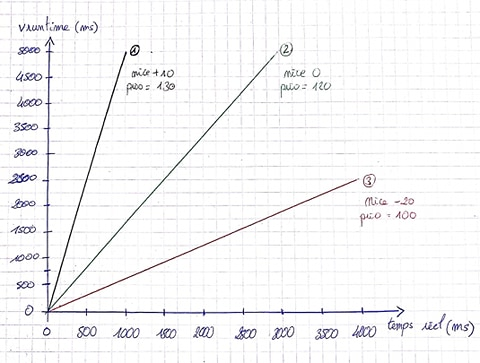
\includegraphics[scale=0.6]{schema_sched.jpg}
	\caption{Relation entre le vruntime et le temps réel en fonction de la priorité}
	\label{fig:sched}
\end{figure}
\\

De part ces faits nous pouvons en déduire que pour prioriser une entité, représentant une tâche détenant un verrou, nous pouvons influencer sur son \verb|vruntime| pour la garder à gauche de l'arbre est assurer une réélection rapide. Cependant cette solution peut présenter plusieurs problèmes. Le code du scheduler reste complexe et une modification aussi importante peut facilement causer des problèmes dans des cas d'exécution non prévu. Étant donné que la valeur \verb|vruntime| se base sur la priorité de l'entité nous avons décidé de ne pas toucher au code du scheduler et d'accélérer les tâches en modifiants habilement leur priorité.

\section*{Scénario}
